\section{Simulation}
\subsection{Vorgehensweise}
Die Daten wurden in 80\% zum Training und 20\% zum Testen aufgeteilt.
Anschließend wurde das "`wahre"' Modell um jeweils ein weiteres Feature erweitert.
Das erweiterte Modell $soil.res = \vec{\beta} * (1,lmoi,temp15,smoi,x)^\text{T}$ wurde mittels ANOVA mit dem "`wahren"' Modell verglichen.
In R berechnete die Funktion \lstinline|anova(realModel, nxtModel)$F[2]| den jeweiligen F-Wert.
Wichtig hierbei war, dass beide Modelle auf den selben Trainingsdaten erstellt wurden und es sich um \it{verschachtelte} Featuremengen handelte.
Die Partitionierung der Daten erfolgte sowohl mittels Kreuzvalidierung als auch mit einem Monte-Carlo-Ansatz.
Bei der 4-fachen Kreuzvalidierung wurden die Daten in vier möglichst gleich großen Partitionen aufgeteilt.
Eine Partition wurde zum Testen des Reproduktionsfehlers verwendet, die Anderen zum Training.
Beim Monte-Carlo-Ansatz wurden 200 mal zufällig 20\% der Daten zum Testen ausgewählt.
Dadurch kann die Wahrscheinlichkeit der Fehlentscheidungen im Bezug auf die Nullhypothese besser geschätzt werden.
Die Ermittlung des Reproduktionsfehlers $\widehat{SPSE}$ erfolgte mittels unabhängigen Testdaten.
Um zu überprüfen, ob sich das Modell überhaupt verbessert hat, wurde die Differenz $\Delta \widehat{SPSE}$ im Bezug auf das Ausgangsmodell berechnet.

\subsection{Auswertung}
\begin{figure}[htbp]
	\centering
	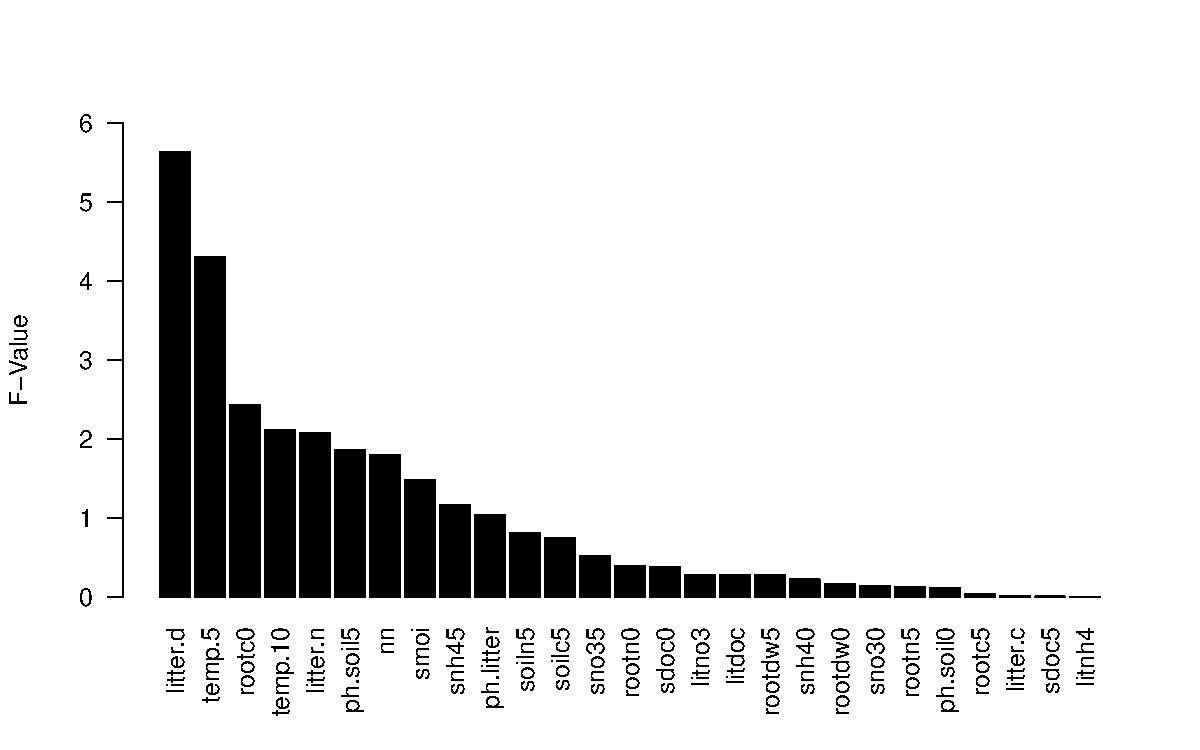
\includegraphics[width=\textwidth]{fig/simul/simul-f.pdf}
	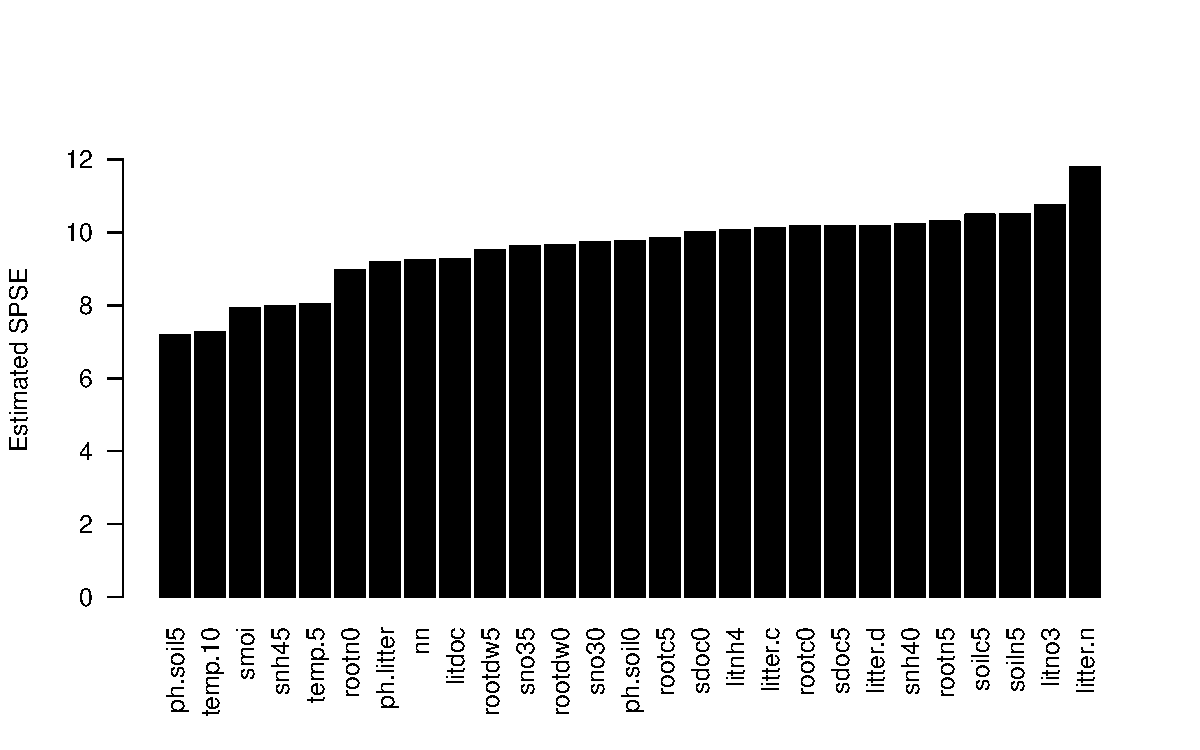
\includegraphics[width=\textwidth]{fig/simul/simul-spse.pdf}
	\caption{\bf{Beispiel einer Simulation.} 
		Das in Kapitel \ref{sec-model} erstellte "`wahre"' Modell wurde um jeweils ein Feature erweitert.
		Dargestellt ist der Fehler \bf{SPSE} und der zugehörige \bf{F-Wert} in Abhängigkeit von der gewählten zusätzlichen Variable in der ersten Runde der Kreuzvalidierung.
		Im Verlaufe der Variablenselektion wird das Modell mit dem höchsten F-Wert gewählt.
		Dies ist allerdings selten das Modell mit dem geringsten Fehler.
	}
	\label{fig-simul-f-spse}
\end{figure}
In Abbildung \ref{fig-simul-f-spse} sind die F-Werte und Fehler bei der Reproduktion von unabhängigen Testdaten gezeigt.
Im Rahmen des Variablenselektionsverfahrens wird jeweils das Feature zum Modell hinzugenommen, welches den größten F-Wert besitzt.
Im diesem Falle wäre das $litter.d$.
Betrachtet man allerdings den erwarteten Reproduktionsfehler $\widehat{SPSE}$, so führt das Hinzunehmen der Variable $ph.soil5$ zum Modell mit minimalen Fehlern.
Hier ist der F-Wert aber um $\approx 3,5$ geringer.
Die Nullhypothese wird hier fälschlicherweise abgelehnt und stattdessen $litter.d$ zum Modell hinzugenommen.
Auch kann es vorkommen, dass eine Zufallsvariable überwiegend Rauschen beinhaltet und sich das Modell dann durch Hinzufügen ebendieser Variable lediglich verschlechtert (Vgl. Abb. \ref{fig-simul-delta-spse}, $\Delta \widehat{SPSE} > 0$)
\\
Nach der Monte-Carlo-Simulation war das Modell mit dem geringsten $\widehat{SPSE}$ stets das Modell mit den 9. höchsten F-Wert.
Während der 200 Simulationen verblieb der Wert unverändert.
Wenn man davon ausgeht, das das erstellte Modell wirklich "`wahr"' ist, so entspricht dies eine Wahrscheinlichkeit zur fehlerhaften Ablehnung der Nullhypothese von $100\%$.
Insgesamt war bei fünf weiteren Features ($temp.10, soilc0, soiln0, snh40$ und $ rootc0$) der p-value stets unter dem Signifikanzniveau.
Hier schlägt das Variablenselektionsverfahren vor, Features einen vollständigen Modell hinzu zufügen.
Unter Annahme der Vollständigkeit des Modells ist dies aber falsch.

\begin{figure}[htb]
	\centering
	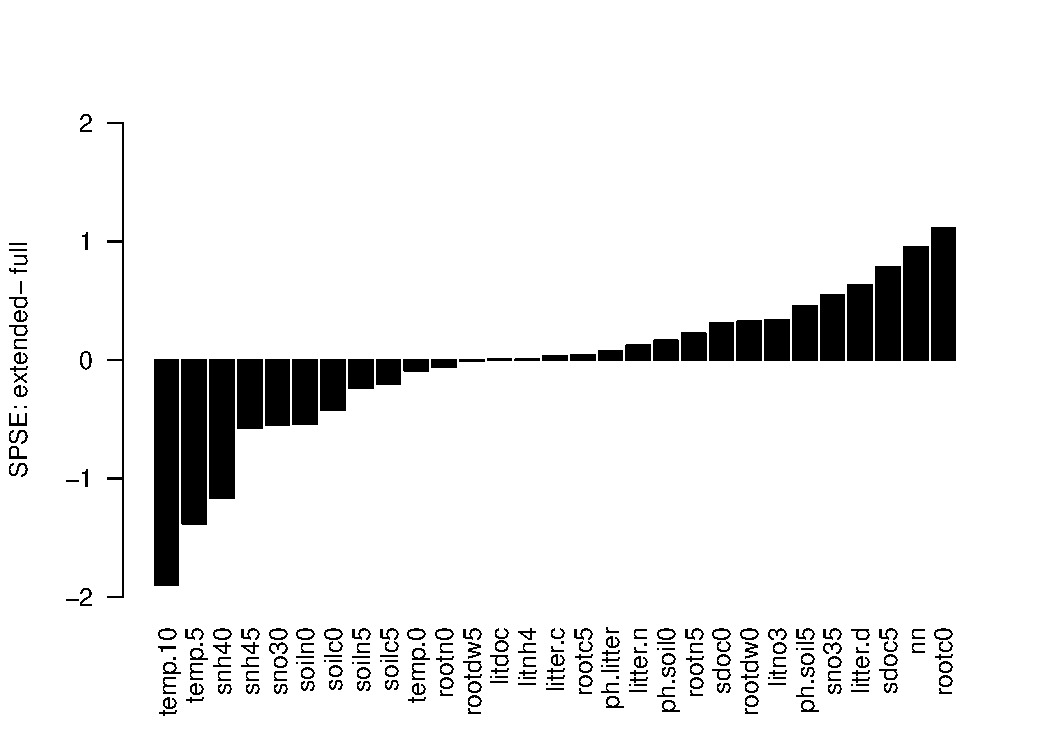
\includegraphics[width=\textwidth]{fig/simul/delta-spse.pdf}
	\caption{\bf{Verbesserung der Modelle.} 
		Dargestellt ist die Differenz $\Delta \widehat{SPSE}$ aus dem „wahren“ und dem erweiterten Modell.
		Positive Werte deuten darauf hin, dass die hinzugefügte Variable dem Modell lediglich Rauschen beifügt.
	}
	\label{fig-simul-delta-spse}
\end{figure}
\\
\begin{figure}[htbp]
	\centering
	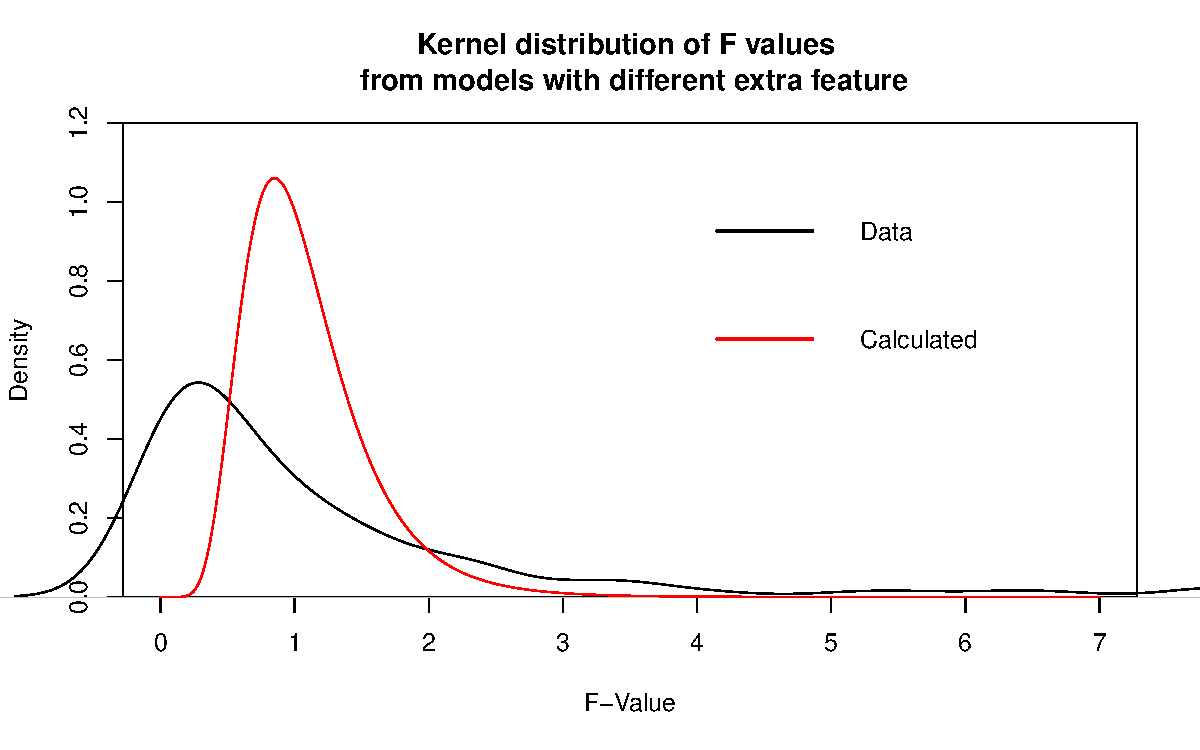
\includegraphics[width=\textwidth]{fig/simul/kernel.pdf}
	\caption{\bf{Approximierte Dichtefunktionen der F-Werte.} 
		Gezeigt ist die Kerneldichtefunktion der F-Werte der Simulationen.
		Die Multimodalität der Funktion deutet auf fehlerhaftes Ablehnen der Nullhypothesen hin.
	}
	\label{fig-simul-kernel}
\end{figure}

Unter der Nullhypothese (Erweitertes Modell ist nicht besser als das "`wahre"' Modell) ist die F-Statistik eine F-verteilte Zufallsvariable.
Die Dichtefunktion der Daten aus der Kreuzüberprüfung (approximiert durch Kernel-Desity) ist nach Abb. \ref{fig-simul-kernel} mitunter stark abweichend.
Die Simulation möchte demnach das wahre Modell erweitern ($H_0$ wird abgelehnt).
Dies führt zu Overfitting, da das Modell bereits als wahr angenommen wurde und demnach keine weiteren Features hinzugefügt werden sollten.

\subsection{Diskussion}
Das Fortführen des Variablenselektionsverfahrens führte zu vielen Ablehnungen der Nullhypothese, obwohl das Modell bereits als vollständig angenommen wurde.
In Anbetracht der Datenlage allerdings lässt sich streiten, ob das Ausgangsmodell wirklich als "`wahr"' bezeichnet werden kann.
Auf jedes Feature kommt maximal ein Datenpunkt.
Damit kann man die Realität nicht abbilden und ein Erstellen eines "`wahren"' Modells erscheint sinnlos.
Ist das wahre Modell nicht bekannt, lässt sich die Wahrscheinlichkeit der fälschlichen Ablehnung von $H_0$ ebenfalls nicht schätzen.
Die Ergebnisse sind demnach mit großer Vorsicht zu genießen.

\subsubsection{Mögliche Gründe der Fehlentscheidungen}
Gemessene Features müssen nicht zwangsläufig von der Bodenatmung statistisch abhängig sein.
Je geringer die Korrelation dieser beiden Zufallsvariablen, desto höher ist die Wahrscheinlichkeit, dass es sich nur um Rauschen handelt.
In diesem Fall sollte diese Variable nicht zum Modell hinzugefügt werden.
Zufälligerweise kann dies aber auch zu hohen F-Werten führen, welches zu fehlerhaften Entscheidungen bei den Hypothesentests führen kann.
Ferner fordert der F-Test normalverteilte Variablen.
Folgt eine Messgröße nicht dieser Verteilung, ist der Test nicht aussagekräftig.
Auch eine nicht repräsentative Stichprobe fälscht das Ergebnis.
Uns lagen lediglich 38 Observationen vor; dies könnte zu gering sein.
Eine fehlerhafte Datenerhebung führt auch zu verfälschten Ergebnissen.
Letztendlich kann der F-Test auch nur zufällig richtig sein.
Ein geringer p-Value schließt keine Fehlentscheidungen aus; sie werden lediglich unwahrscheinlicher.

\subsubsection{Auswirkungen der Designmatrix auf die Fehlentscheidungen}
In der Monte Carlo-Simulation wurden 200 unterschiedliche Teilmengen des Datensatzes als Trainingsdaten verwendet.
Die Designmatrix kann also in jeder Runde leicht anders ausfallen.
In jeder Einzelsimulation jedoch war stets $Temp.10$ das Feature mit dem höchsten F-Wert.
Die Wahl der Trainingsdaten führte zwar zu leicht unterschiedlichen Koeffizienten $\beta_i$; die Entscheidung des nächsten Features jedoch war stets die selbe.
Die Messungen sind demnach statistisch voneinander unabhängig.


